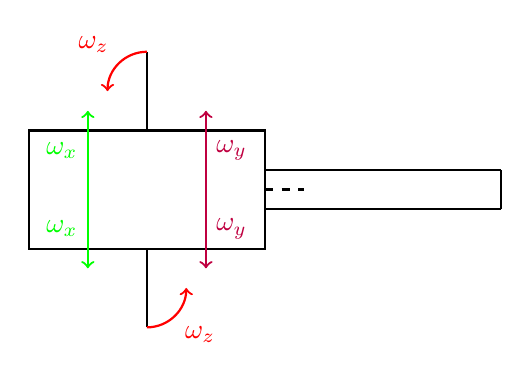
\begin{tikzpicture}

% Draw the tractor
\draw[thick] (0,0) rectangle (3,1.5);
\draw[thick] (1.5,1.5) -- (1.5,2.5); % Front axle
\draw[thick] (1.5,0) -- (1.5,-1); % Rear axle

% Draw the trailer
\draw[thick] (3,0.5) -- (6,0.5);
\draw[thick] (3,1) -- (6,1);
\draw[thick] (6,0.5) -- (6,1); % Rear of the trailer

% Draw the coupling
\draw[thick, dashed] (3,0.75) -- (3.5,0.75);

% Angular velocities
\draw[->, red, thick] (1.5,2.5) arc[start angle=90, end angle=180, radius=0.5] node[midway, above left] {$\omega_z$};
\draw[->, red, thick] (1.5,-1) arc[start angle=270, end angle=360, radius=0.5] node[midway, below right] {$\omega_z$};

% Annotations for roll and pitch (using 3D-like perspective)
\draw[->, green, thick] (0.75,0.75) -- (0.75,1.75) node[midway, left] {$\omega_x$};
\draw[->, purple, thick] (2.25,0.75) -- (2.25,1.75) node[midway, right] {$\omega_y$};

% Additional 3D-like arrows for better visualization
\draw[->, green, thick] (0.75,0.75) -- (0.75,-0.25) node[midway, left] {$\omega_x$};
\draw[->, purple, thick] (2.25,0.75) -- (2.25,-0.25) node[midway, right] {$\omega_y$};

\end{tikzpicture}